\section{Economic Rationale}

\subsection{Current Solutions}

	As is evident, sleep apnea, particularly obstructive sleep apnea (OSA)
affects a significant proportion of the population and is worthy of
attention. The current available diagnosis options for sufferers or
potential sufferers are limited, expensive, invasive and realtively
inaccessible. We outline below the most common sources of help and
diagnosis for potential sufferers:
	\begin{itemize}
	\item NHS - GP check-up, home devices and polysomnography (PSG)
	\item Commercial home-testing devices
	\item Other possible future options such as mobile sleep apps and non-contact
health sensing technologies
	\end{itemize}

\subsubsection{NHS}

According to the NHS guidelines, patients who believe they may be suffering from sleep apnea can schedule a visit to their GP. The GP will ask a few questions to determine the likelihood of apnea, along with a physical examination that includes a blood pressure (BP) test and a hypothyroidism test, to determine whether an underactive thyroid gland is the reason for the patient's tiredness. The patient can then choose if he/she would like to be observed for one night in a sleep
centre, or would like to be given a monitoring device to wear at home when sleeping. Those who opt for a home sleep study are required to visit the sleep centre at a convenient time to collect and learn how to use the portable recording equipment. These include breathing sensors, heart rate monitors and oxygen sensors. Information from the device can be analysed on the next visit and further action, such as referring to a sleep centre can be taken \cite{nhsmain,nhsdiag}.

Observation at a sleep centre is done through polysomnography (PSG). This involves electrodes being placed on the face, scalp and above the lips, and bands being placed around the chest and abdomen. Additionally, sensors are placed on the legs and an oxygen sensor is attached to a finger. The tests carried out during a PSG include:

	\begin{itemize}
	\item Electro-encephalography (EEG)
	\item Electromyography (EMG)
	\item Recording of thoracoabdominal movements
	\item Recording of oronasal airflow
	\item Pulse Oximetry
	\item Electrocardiography (ECG)
	\item Sound and Video Recording
	\end{itemize}

The data from these tests is used to positively diagnose obstructive sleep apnea and a treatment regimen is then decided upon and enforced by the healthcare professional \cite{nhsdiag}. For the purposes of this report, we shall not delve into the treatment of OSA - we concern ourselves with the diagnosis process and how we can improve it.


\subsubsection{Commercial home-testing devices}

While these devices are more commmon in the United States, they are also available in the UK, and can be purchased if desired without visiting a GP. An example of such home-testing devices is the AccuSom\textsuperscript{\textregistered{}} test from NovaSom Inc. \cite{novasom1,novasom2}, pictured below: 

\begin{figure}[!ht]
\centering
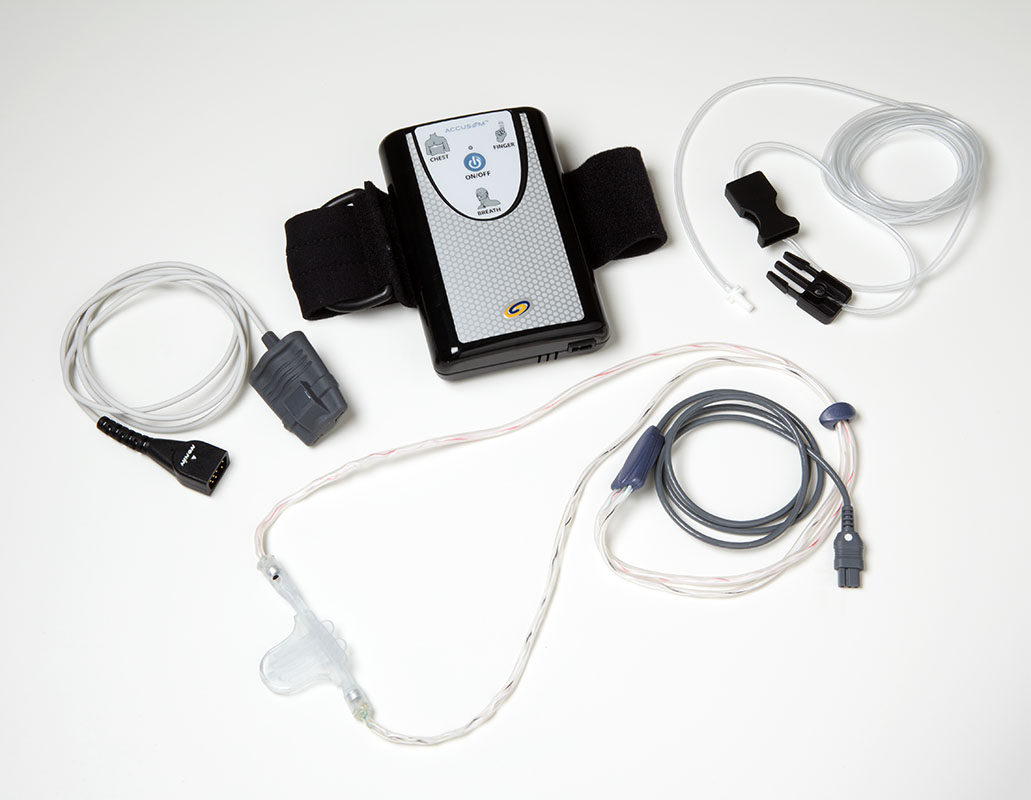
\includegraphics[width=0.5\textwidth]{drawings/Novasom}
\caption{AccuSom\textsuperscript{\textregistered{}} \cite{novasom2}}
\label{fig:Novacom}
\end{figure}

The prevalence of such tests in the U.S. points towards the increasing
unfeasiblity of sleep centre tests for simple diagnosis of OSA, and
is an indication of where the diagnosis process is headed in the future,
in the U.K. as well as around the world. The economic reasons for
the trend are clear. On average, a single night at a sleep centre
and the associated tests could cost from \$800 to \$3000 in the U.S \cite{wsjhometest}.
(figures for the NHS in the U.K. are more difficult to find, but should
be comparable) The home tests can be administered at a fraction of
that price, ranging from \$200 to \$600 \cite{wsjhometest}. Moreover, sleep centre tests
are extremely inconvenient for the patients, and hence should be administered
towards the later stages of the diagnosis process. The use of home-testing
devices also allows a larger percentage of the population to be able
to test for OSA, which is desirable given that around 5\% suffer
from undiagnosed OSA \cite{nhsmain}.


\subsubsection{Other options}

The trend towards greater user independence in OSA diagnosis is further
observed through two major related breakthroughs - the rise of mobile
sleep apps and the development of non-contact health sensing technologies.

The popularity of sleep monitoring apps in the iOS and Android App
stores illustrates an increasing interest among smartphone users in
their sleep patterns. Currently, such apps use the accelerometers
and microphones to detect movements and noises from the users while they sleep, and use relatively simple algorithms to determine which stage of sleep the user is in. In addition, some apps come with additional headsets or headbands that track electrical impulses and measure the user's activity more accurately. The alarm clock function is activated only when the user is in light sleep (within a reasonable time window) to ensure he/she is woken up feeling energised \cite{currentapps}. Some examples of such apps are:

\begin{itemize}
\item Sleep Cycle (iOS) - \$1
\item Sleep Bot Tracker (Android) - Free
\item Wakemate - \$60
\item Lark - \$99
\item Zeo Sleep Manager Mobile - \$99
\item Sleep Tracker Elite - \$149 
\end{itemize}

The development of non-contact health sensing technologies holds promise as well. Recently, Xerox and Manipal University Hospital in India announced a collaboration to develop such techonologies at Xerox's research centre in Bangalore \cite{xerox1, xerox2}. Using image and signal processing algorithms, the collaboration aims to determine health indicators in a non-invasive manner, and such that monitoring can take place remotely \cite{xerox1}. The clear trend of health monitoring towards non-invasive methods and the increasing use of algorithms to supplement health care and diagnosis efforts is set to gain even more momentum as healthcare professionals begin to embrace 'big data' \cite{bigdata}.

\subsection{Proposed App - Where it fits in}

The need for an app that is able to diagnose OSA from a mobile platform, using non-invasive techniques is clear from the current diagnosis solutions and trends. While there has been a shift towards cheaper home-testing devices before necessitating a visit to a sleep centre, the fact remains that even at \$200, these tests are not inexpensive. What if we could create a means for diagnosing OSA without the need for cumbersome and invasive sensors, that could be accessed by anyone with a smartphone, at a negligible cost compared to a home-testing system? Those who have doubts over their sleep habits, but are too busy for a GP visit and do not want to spend money unnecessarily on a home-testing system could try the app and move on to pursue the matter more seriously if the results from the app suggested a need to do so. Since machine learning algorithms will be used in the processing of the data, the app has the potential to continuously improve in accuracy and, eventually, could outperform the home-testing devices. The development of image processing technology that could remove the need for invasive monitoring, especially in neonatal care, by Manipal University Hospital and Xerox sets a precedent and raises the possibility of diagnosing OSA without the need for sensors being placed around the body.


\subsection{Advantages of proposed app}

The advantages of the proposed smartphone app, that will use machine learning algorithms to accurately diagnose OSA using non-invasive mobile phone sensors, are numerous. Firstly, such an app, if utilised as a precursor to home-testing systems and sleep centres, could result in significant cost savings for both the healthcare provider and the patient. From the point of view of the NHS, savings from performing polysomnographies only on those who really need it would be substantial. Moreover, some of the functions such as collecting information about the patient can be done through the app using questionnaires to save time for the doctors. From the point of view of the patients, not having to schedule visits to the GP for collecting and returning home-testing kits would result in a larger number of users for the app than would otherwise have been the case.
This brings us to another advantage of using the mobile app - accessibility. Given that 65 \% of people over 65 in the U.K. have OSA \cite{nhsmain}, along with a significant proportion of middle-aged men and women, and that the condition often goes undiagnosed, it is essential to reach out to as many users as possible. The best way to do so is through mobile phones. The number of smartphone users is projected to increase globally from 1.75 billion in 2014 to almost 2.5 billion by 2017 \cite{phoneusers}. The graph below highlights the growth of mobile phone users worldwide:

\begin{figure}[!ht]
\centering
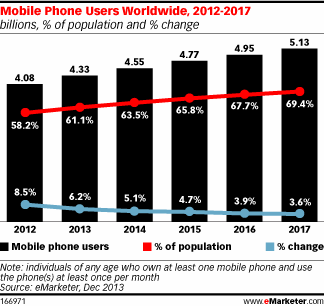
\includegraphics[width=0.5\textwidth]{drawings/mobilephoneusers.png}
\caption{Mobile Phone Users 2012 - 2017 \cite{phoneusers}}
\label{fig:mobilephoneusers}
\end{figure}

This highlights the potential for the app, and smartphone-aided diagnosis in general, not just in the U.K. but in other developing countries as well, where access to a sleep centre may not be as readily available.

The advantage that the proposed app holds over existing mobile phone apps is that it is specifically for diagnosing OSA - it is meant for medical purposes as opposed to general sleep cycle monitoring. This means that it does not compete with the above-mentioned apps, but serves a distinct purpose which is not possible in the other apps. Moreover, the use of machine learning algorithms in the app means that there is potential for the app to improve in accuracy over time as the amount and quality of training data used is improved. With every update, the app can become better at diagnosing OSA using only non-invasive methods.

In conclusion, the rationale for the project to develop such an app is clear. If developed, the app is viable as a supplementary service by the NHS and can improve the diagnosis of OSA in adults in the U.K. dramatically by reaching out to a wider audience and simultaneously result in savings for the NHS. It can also be further developed for use internationally, by those in developing countries in the future.
